\documentclass[draft=false
              ,paper=a4
              ,twoside=false
              ,fontsize=11pt
              ,headsepline
              ,BCOR10mm
              ,DIV11
              ]{scrbook}
\usepackage{graphicx}
\usepackage[ngerman,english]{babel}
%% see http://www.tex.ac.uk/cgi-bin/texfaq2html?label=uselmfonts
\usepackage[T1]{fontenc}
%\usepackage[utf8]{inputenc}
\usepackage[latin1]{inputenc}
\usepackage{libertine}
\usepackage{pifont}
\usepackage{microtype}
\usepackage{textcomp}
\usepackage[german,refpage]{nomencl}
\usepackage{setspace}
\usepackage{makeidx}
\usepackage{listings}
\usepackage{natbib}
\usepackage[ngerman,colorlinks=true]{hyperref}
\usepackage{soul}
\usepackage{hawstyle}
\usepackage{lipsum} %% for sample text

%% define some colors
\colorlet{BackgroundColor}{gray!20}
\colorlet{KeywordColor}{blue}
\colorlet{CommentColor}{black!60}
%% for tables
\colorlet{HeadColor}{gray!60}
\colorlet{Color1}{blue!10}
\colorlet{Color2}{white}

%% configure colors
\HAWifprinter{
  \colorlet{BackgroundColor}{gray!20}
  \colorlet{KeywordColor}{black}
  \colorlet{CommentColor}{gray}
  % for tables
  \colorlet{HeadColor}{gray!60}
  \colorlet{Color1}{gray!40}
  \colorlet{Color2}{white}
}{}
\lstset{%
  numbers=left,
  numberstyle=\tiny,
  stepnumber=1,
  numbersep=5pt,
  basicstyle=\ttfamily\small,
  keywordstyle=\color{KeywordColor}\bfseries,
  identifierstyle=\color{black},
  commentstyle=\color{CommentColor},
  backgroundcolor=\color{BackgroundColor},
  captionpos=b,
  fontadjust=true
}
\lstset{escapeinside={(*@}{@*)}, % used to enter latex code inside listings
        morekeywords={uint32_t, int32_t}
}
\ifpdfoutput{
  \hypersetup{bookmarksopen=false,bookmarksnumbered,linktocpage}
}{}

%% more fancy C++
\DeclareRobustCommand{\cxx}{C\raisebox{0.25ex}{{\scriptsize +\kern-0.25ex +}}}

\clubpenalty=10000
\widowpenalty=10000
\displaywidowpenalty=10000

% unknown hyphenations
\hyphenation{
}

%% recalculate text area
\typearea[current]{last}

\makeindex
\makenomenclature

\begin{document}
\selectlanguage{ngerman}

%%%%%
%% customize (see readme.pdf for supported values)
\HAWThesisProperties{Author={Daniel Kirchner}
                    ,Title={Skalierbare Datenanalyse mit Apache Spark}
										,SubTitle={Architekturanalyse und Performancetests in verschiedenen Anwendungsf�llen}
                    ,EnglishTitle={Scalable Data Analysis with Apache Spark}
                    ,ThesisType={Bachelorarbeit}
                    ,ExaminationType={Bachelorpr�fung}
                    ,DegreeProgramme={Bachelor of Science Angewandte Informatik}
                    ,ThesisExperts={Prof. Dr. Kahlbrandt \and Prof. Dr. Zweitpr�fer}
                    ,ReleaseDate={1. Januar 2345}
                  }

%% title
\frontmatter

%% output title page
\maketitle

\onehalfspacing

%% add abstract pages
%% note: this is one command on multiple lines
\HAWAbstractPage
%% German abstract
{Schl�sselwort 1, Schl�sselwort 2}%
{Dieses Dokument \ldots}
%% English abstract
{keyword 1, keyword 2}%
{This document \ldots}

\newpage
\singlespacing

\tableofcontents

\newpage
%% enable if these lists should be shown on their own page
%%\listoftables
%%\listoffigures
\lstlistoflistings

%% main
\mainmatter
\onehalfspacing
%% write to the log/stdout
\typeout{===== File: chapter 1}
%% include chapter file (chapter1.tex)
%%\include{chapter1}

%%%%
%% add some text to generate a sample document
\chapter{Einf\"uhrung}

\section{Motivation}

Die Entwicklung und Verbesserung von Frameworks zur Verarbeitung gro�er Datenmengen ist zur Zeit hochaktuell und sehr im Fokus von Medien und Unternehmen [VERWEIS]. Verschiedene Programme und Paradigmen konkurrieren um die schnellste, bequemste und stabilste Art gro�en Datenmengen einen gesch�ftsf�rdenden Nutzen abzuringen.
\break

Unter dem Begriff "`gro�e Datenmengen"' oder "`Big Data"' werden solche Datenmengen zusammengefasst, die die Kriterien Volume, Velocity, Variety [VERWEIS, Doug Laney] erf�llen oder "`Datenmengen, die nicht mehr unter Auflage bestimmter SLAs auf einzelnen Maschinen verarbeitet werden k�nnen"' [VERWEIS, Hadoop/Yarn Entwickler].

Als Unternehmen, das fr�h mit solchen Datenmengen konfrontiert war implementierte Google das Map-Reduce Paradigma [VERWEIS] als Framework zur Ausnutzung vieler "`Mittelklasse"'-Rechner um Webseiten einzustufen und f�r andere Aufgaben [VERWEIS]. 

In Folge der Ver�ffentlichung ihrer Idee im Jahr 2005 [VERWEIS] wurde Map-Reduce in Form der OpenSource Implementation Hadoop (gemeinsam mit einer Implementation des Google File Systems GFS, u.a.) [VERWEIS] zum de-facto Standard f�r Big-Data-Analyseaufgaben [VERWEIS?].
\break

Map-Reduce als Programmierparadigma zur effizienten Stapelverarbeitung gro�er Datenmengen zeigt jedoch in vielen Anwendungsf�llen Schw�chen:
\begin{itemize}
	\item Daten, die in hoher Frequenz ver�ndert werden erfordern das st�ndige Neustarten eines Map-Reduce-Jobs. 	Iterative Algorithmen sind also nicht vorgesehen.
	\item Die Anfrage an ein solches System erfolgt in Form von kleinen Programmen. Dieses Verfahren ist offensichtlich nicht so deklarativ und leicht erlernbar wie SQL-Anfragen an klassische Datenbanken.
\end{itemize}

In der Folge entstanden viele Ans�tze dieses Paradigma zu ersetzen, zu erg�nzen oder durch �bergeordnete Ebenen und High-Level-APIs zu vereinfachen.

\begin{itemize}
	\item {[}VERWEIS: A survey of large scale...{]} oder Aufz�hlung.
\end{itemize}

Eine der Alternativen zu der Map-Reduce-Komponente in Hadoop die "`general engine for large-scale data processing"' Apache Spark.

Zum aktuellen Zeitpunkt hat das Interesse an Apache Spark das Apache Hadoop Framework bereits �berholt:
\break

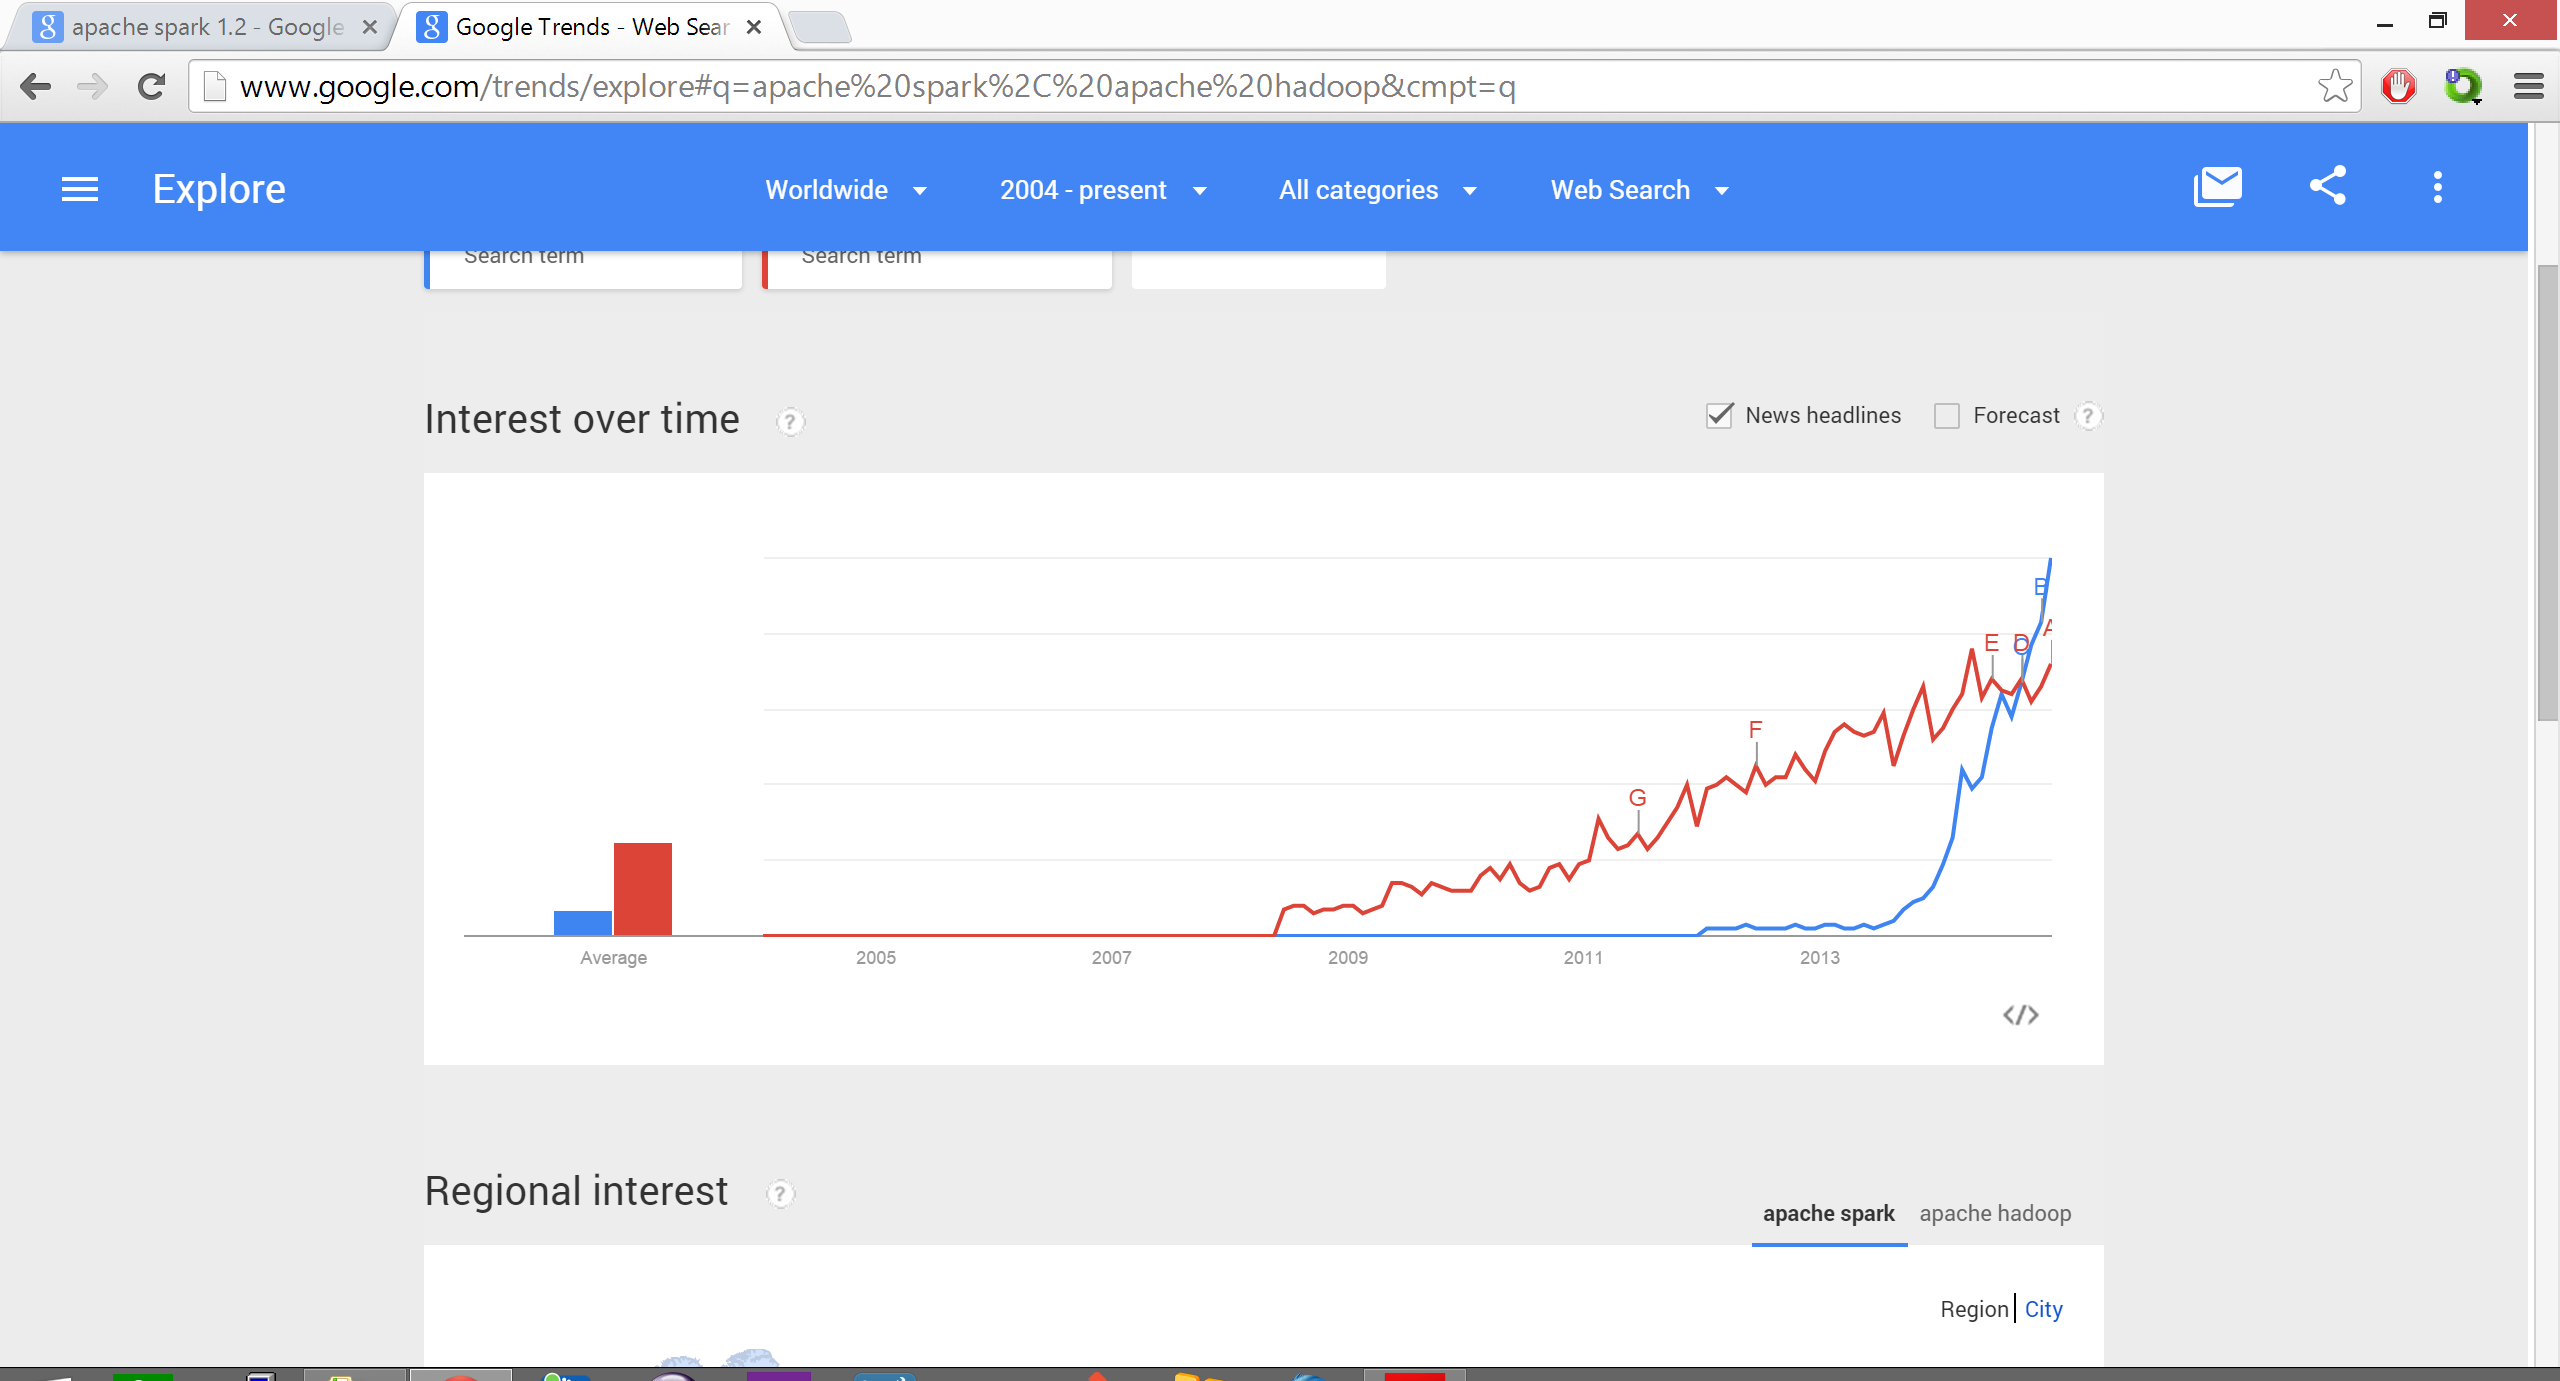
\includegraphics[scale=0.4]{bilder/trends_spark_vs_hadoop.PNG}

\section{Kontextabgrenzung}

\section{Verwandte Produkte}

\subsection{\"Uberblick}
\subsection{YARN}
\subsection{Flink}
\subsection{...}

\chapter{Vorstellung von Apache Spark}

\section{\"Ubersicht}
\subsection{Architektur�bersicht}
\subsection{Standardbibliotheken}
\subsubsection{Spark SQL}
\subsubsection{MLlib}
\subsubsection{Streaming}
\subsubsection{GraphX}

\section{Wesentliche Konzepte}
\subsection{Abgrenzung zu Hadoop}
\subsection{Resilient Distributed Datasets}


\chapter{Vorstellung des Beispiels}
\section{Aufgabenbeschreibung}
\section{L\"osungsidee}
\subsection{1. Schritt: \"Ahnlichkeitsma{\ss} f�r W\"orter erzeugen}
\subsection{2. Schritt: Echtzeitbewertung von Textnachrichten aus einem Datenstrom}


\chapter{Implementation und Bewertung}
\section{Betriebsumgebung}
Die Wahl einer Betriebsumgebung f�r Cluster-Computing-Frameworks stellt besondere Anforderungen. Obwohl Installationen einer lauff�higen Instanz von Apache Spark auch f�r einzelne Maschinen m�glich ist, werden solche Setups einer Demonstration und Untersuchung von verteiltem Rechnen offensichtlich nicht gerecht.

Auf der anderen Seite bringen verteilte und auf physikalischen Rechnern laufende Installationen zus�tzliche Probleme mit. Ausf�lle von Hardwarekomponenten auf Rechenknoten und Netzwerken, Stromkosten f�r Betrieb und K�hlung, sowie Beschaffungs- oder Mietkosten f�r R�umlichkeiten und Komponenten sind nur die offensichtlichsten.
\break

Im Rahmen dieser Arbeit sollen Konzepte demonstriert und bewertet werden. Ein produktionstaugliches System ist  nicht gefordert. Es ergeben sich die folgenden Vorgaben. 
\break

Anforderungen:
\begin{itemize}
	\item echte Verteilung der Komponenten
	\item volle Kontrolle �ber die lokalen Abl�ufe
\end{itemize}

Keine Anforderungen:
\begin{itemize}
	\item hohe Performance
	\item authentische Bedingungen eines Rechenzentrums
\end{itemize}

Gem�� dieser Anforderungen kommt ein KVM-virtualisierter Host zum Einsatz der als Plattform f�r eine Cloud Computing Software dient, um ein kleines Cluster von virtuellen Maschinen zu Verf�gung zu stellen.
\break

Technische Daten des Hosts
\begin{itemize}
	\item CPU Intel� Xeon� E5-2670V2
	\item 4 dedizierte Kerne
	\item 16GB DDR3 RAM
	\item Betriebssystem Fedora 20 GNU/Linux
	\item Cloud Software OpenStack (Release Juno)
\end{itemize}

Das Cluster selbst besteht aus 3 gleichartigen virtuellen Maschinen innerhalb eines OpenStack Tenants und dem Host selbst. Um die untersuchte Installation in andere Betriebsumgebungen zu bringen oder schnell wiederherstellen zu k�nnen, sind die Installationen der Apache Spark Komponenten jeweils in Docker Containern (basierend auf LXC) durchgef�hrt.
Dadurch daraus ergeben sich drei Laufzeitumgebungen f�r den Entwicklungs- und Untersuchungsprozess:
\break

\begin{itemize}
	\item Lokale Single-Node-Installation: Exploration, Entwicklung, Debugging
	\item {[}Docker{]} Virtuelles Cluster auf einzelner physiklischen Maschine: Entwicklung und Debugging im verteilten Betrieb
	\item {[}Docker{]} Virtuelles Cluster auf verteilten physikalischen Maschinen: Performance-Messungen, Analyse von Skalierungsverhalten
\end{itemize}


Technische Daten der virtuellen Cluster-Knoten
\begin{itemize}
	\item 2 virtuelle CPUs
	\item 2GB RAM
	\item Betriebssystem CoreOS
	\item Netzwerkvirtualisierung mit der OpenStack-Komponente Neutron
\end{itemize}

\subsection{Verteilungsdiagramm}


\section{Architektur�bersicht}
\section{Architekturdetails}
\subsection{Modell f\"ur \"Ahnlichkeit von W\"ortern mit MLlib erzeugen}
\subsection{Einlesen von Nachrichten aus dem Twitter Livestream}
\subsection{Verarbeiten und Bewerten der Nachrichten}
\section{Bewertung der Verfahren}

\chapter{Schlussbetrachtung}
\section{Kritische W\"urdigung der Ergebnisse}
\section{Ausblick und offene Punkte}

%%\lipsum

See also \cite{sample_bib}.
%%%%

%% appendix if used
%%\appendix
%%\typeout{===== File: appendix}
%%\include{appendix}

% bibliography and other stuff
\backmatter

\typeout{===== Section: literature}
%% read the documentation for customizing the style
\bibliographystyle{dinat}
\bibliography{sample}

\typeout{===== Section: nomenclature}
%% uncomment if a TOC entry is needed
%%\addcontentsline{toc}{chapter}{Glossar}
\renewcommand{\nomname}{Glossar}
\clearpage
\markboth{\nomname}{\nomname} %% see nomencl doc, page 9, section 4.1
\printnomenclature

%% index
\typeout{===== Section: index}
\printindex

\HAWasurency

\end{document}
